
\documentclass[aspectratio=169,11pt]{beamer}
\usetheme{metropolis}
\usepackage{amsmath,amssymb}
\usepackage{booktabs}
\usepackage{graphicx}
\usepackage{tikz}
\graphicspath{{figures/}}
%\setbeamertemplate{frame footer}{A.\ J.\ Valbuena -- SEAQT vs Advantage2}
% ---------- Qubit-graph drawing style ----------
\tikzset{
  qubit/.style={circle, draw=blue!60!black, fill=blue!12, thick,
                minimum size=7mm, font=\footnotesize},
  qcoupling/.style={line width=1pt, draw=blue!55!black}
}

\title{Non-Equilibrium Evolution Using the Steepest Entropy Ascent Quantum Thermodynamics Framework with Applications to Quantum Annealing Hardware}
\author{Andrés J.\ Valbuena Villamil}
\institute{
  \inst{1} Jülich Supercomputing Centre, Germany. \qquad -- \qquad advisor: Dr. Jhon Alejandro Montañez Barrera  
  \and
  \inst{2} University of Guanajuato, Mexico. \qquad -- \qquad advisor: Dr. César Eduardo Damián Asencio
}
\date{\today}

\begin{document}

\maketitle


% ================= Objective =================
\begin{frame}{Research Objective}
  \begin{block}{}
    Evaluate the predictive capability of the \textbf{SEAQT} (Steepest
    Entropy Ascent Quantum Thermodynamics) formalism for describing the
    \textbf{non-equilibrium evolution} of systems implemented on the
    D-Wave Advantage2 quantum annealing processor \textbf{``JUPSI''} at
    Forschungszentrum J\"ulich.
  \end{block}
 
\end{frame}
 
% ================= Motivation =================
\begin{frame}{Motivation: Real Annealers Are Open Quantum Systems}
  \begin{itemize}
    \item Quantum annealers are never perfectly isolated from their
      environment -- real hardware shows deviations from ideal,
      closed-system (unitary) dynamics.
    \item \textbf{King et al.\ 2022} (D-Wave, 2000-qubit Ising chain,
      arXiv:2202.05847) demonstrated this directly: for \emph{fast}
      anneals, the hardware matches closed-system quantum theory with
      \textbf{no fitting parameters} -- genuine coherent evolution.
    \item But for \emph{slower} anneals, they observe \textbf{anti-Kibble-Zurek}
      behavior -- a clear signature of thermal/open-system effects that
      closed-system theory cannot produce.
  \end{itemize}
  
\end{frame}
% ------------------------------------------------------------------ 2. SEAQT
\section{Steepest Entropy Ascent Quantum Thermodynamics, SEAQT}

\begin{frame}{SEAQT Framework}
Non-linear extension of the schr\"odinger (Von Neumann) equation, which describes the evolution of a quantum system following the steepest entropy ascent path, in accordance with the second law of thermodynamics. 
  \[
    \dot\rho = \underbrace{-\frac{i}{\hbar}[H(t),\rho]}_{\text{unitary (annealing)}} \;+\; \underbrace{\mathcal{D}}_{\text{SEAQT dissipator}}
  \]
 The dissipator term takes two forms in this project:
 \begin{columns}
     \column{0.45 \textwidth}\[\mathcal{D}_{global}= -\frac{\beta}{2\tau}\{\Delta \hat F,\rho\}\] \[ 
    \Delta \hat F = (\hat H - \langle  \hat H \rangle ) - \frac{1}{\beta}(\hat S - \langle \hat S\rangle) \] 
    \column{0.45 \textwidth}
    \[
    \mathcal{D}_{local} = -\sum_{J = 1}^{M} \frac{1}{\tau_J}\hat{D}_J\otimes\hat{\rho}_{\bar{J}}
  \]
  \[
    \hat{D}_J = \hat{\rho}_J \ln \hat{\rho}_J - \beta_R \langle f \rangle_J \hat{\rho}_J +\frac{1}{2} \beta_R \{ \hat{H}_J , \hat{\rho}_J\}
  \]
 \end{columns}
  \note{Keep it light: one equation, what it does, one parameter.}
\end{frame}

% ------------------------------------------------------------------ 3. method
\section{Method}

\begin{frame}{Problems: six-qubit rings and chains, $h=0$}
  \begin{columns}[T]
    \column{0.5\textwidth}
    \begin{itemize}
    \item \textbf{Exploratory phase:} t$_a$ $\in [5,20000]$ ns, 1000 reads for each value of t$_a$
    \item \textbf{Refinement phase:} t$_a$ $\in [5,145]$ ns, where both coherent and begins of floor regimes can be observed. 8000 reads for each value of t$_a$ 
      \item Ring (6-cycle) and chain (same qubits, closing coupler removed); both signs of $J$.
      \item $J$ chosen so the quantum/classical crossing $A(s_c)=B(s_c)\,|J|$ sits at an energy
            $n\cdot k_BT/h$ ($T=20$ mK, $k_BT/h=417$ MHz).
    \end{itemize}
    \column{0.45\textwidth}
     \centering
      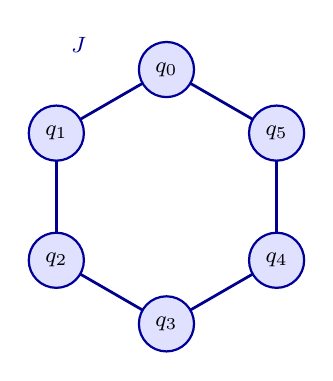
\begin{tikzpicture}[scale=0.95]
        \foreach \i in {0,...,5} {
          \coordinate (q\i) at ({90+60*\i}:1.7);
        }
        \foreach \i [evaluate=\i as \j using {int(mod(\i+1,6))}] in {0,...,5} {
          \draw[qcoupling] (q\i) -- (q\j);
        }
        \foreach \i in {0,...,5} {
          \node[qubit] at (q\i) {$q_{\i}$};
        }
        \node[qcoupling, draw=none, font=\footnotesize\itshape, blue!55!black]
          at ({90+30}:2.35) {$J$};
      \end{tikzpicture}
      \vspace{4pt}
      \textbf{Ring} (6-cycle)\\
      \footnotesize 6 couplings, periodic boundary conditions
      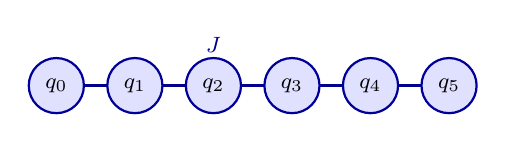
\begin{tikzpicture}[scale=0.95]
        \foreach \i in {0,...,5} {
          \coordinate (c\i) at (\i*1.05, 0);
        }
        \foreach \i [evaluate=\i as \j using {int(\i+1)}] in {0,...,4} {
          \draw[qcoupling] (c\i) -- (c\j);
        }
        \foreach \i in {0,...,5} {
          \node[qubit] at (c\i) {$q_{\i}$};
        }
        \node[font=\footnotesize\itshape, blue!55!black] at (2.1,0.55) {$J$};
      \end{tikzpicture}
 
      \vspace{4pt}
      \textbf{Open chain} (5 edges)\\
      \footnotesize 5 couplings, no periodic boundary
  \end{columns}
  %\note{Annealing people will ask why these J: they place the crossing at a controlled multiple of the thermal energy.}
\end{frame}

\begin{frame}{Simulation: exact $64\times64$ density matrix}
  \begin{itemize}
    \item Hamiltonian $H(s) = -\tfrac{A(s)}{2}\sum_i\sigma^x_i + \tfrac{B(s)}{2}\sum_{\langle ij\rangle}J_{ij}\sigma^z_i\sigma^z_j$,
          real Advantage2 schedule.
    \item Units: schedule in GHz ($E/h$) $\Rightarrow$ $H_{\text{ang}}=2\pi H_{\text{GHz}}$ in rad/ns.
    \item \textbf{Ideal case} = closed SEAQT (no dissipator): exact unitary evolution. Dissipative: factorized
          integrator, positive by construction.
    \item Observable: $P_{GS}$, probability of the classical ground states, vs.\ $t_a$.
  \end{itemize}
\end{frame}

\begin{frame}{Validation: Landau--Zener regime of King et al.\ (2022)}
  \begin{columns}[c]
    \column{0.55\textwidth}
    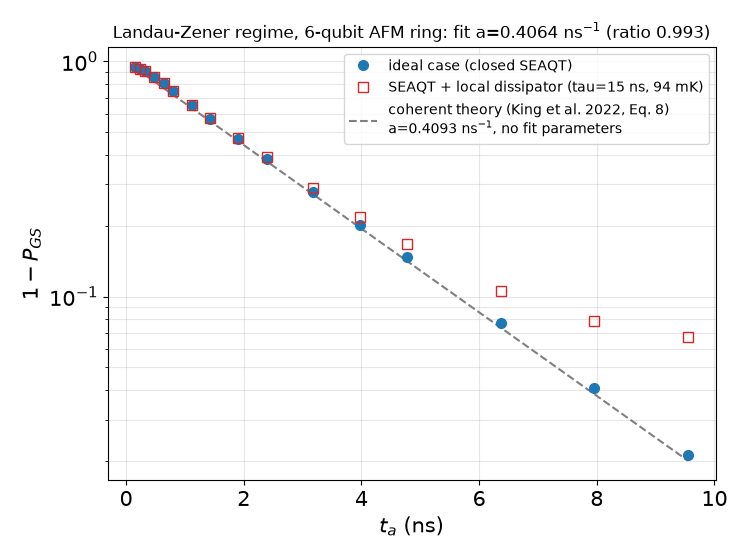
\includegraphics[width=\linewidth]{king_validation.png}
    \[ 1- P_{GS}=e^{-at_a}, \quad a=2\pi^3bL^{-2}\]
    \column{0.42\textwidth}
    \begin{itemize}
      \item 6-qubit AFM ring, coherent regime.
      \item Fitted decay rate $a=0.4064$ ns$^{-1}$ vs.\ King's Eq.~8: $0.4093$ ns$^{-1}$ (ratio $0.993$),
      \item The simulation reproduces a known coherent-annealing result before we compare with hardware.
    \end{itemize}
  \end{columns}
\end{frame}
\begin{frame}{Advantage2 shows three regimes}
  \centering
  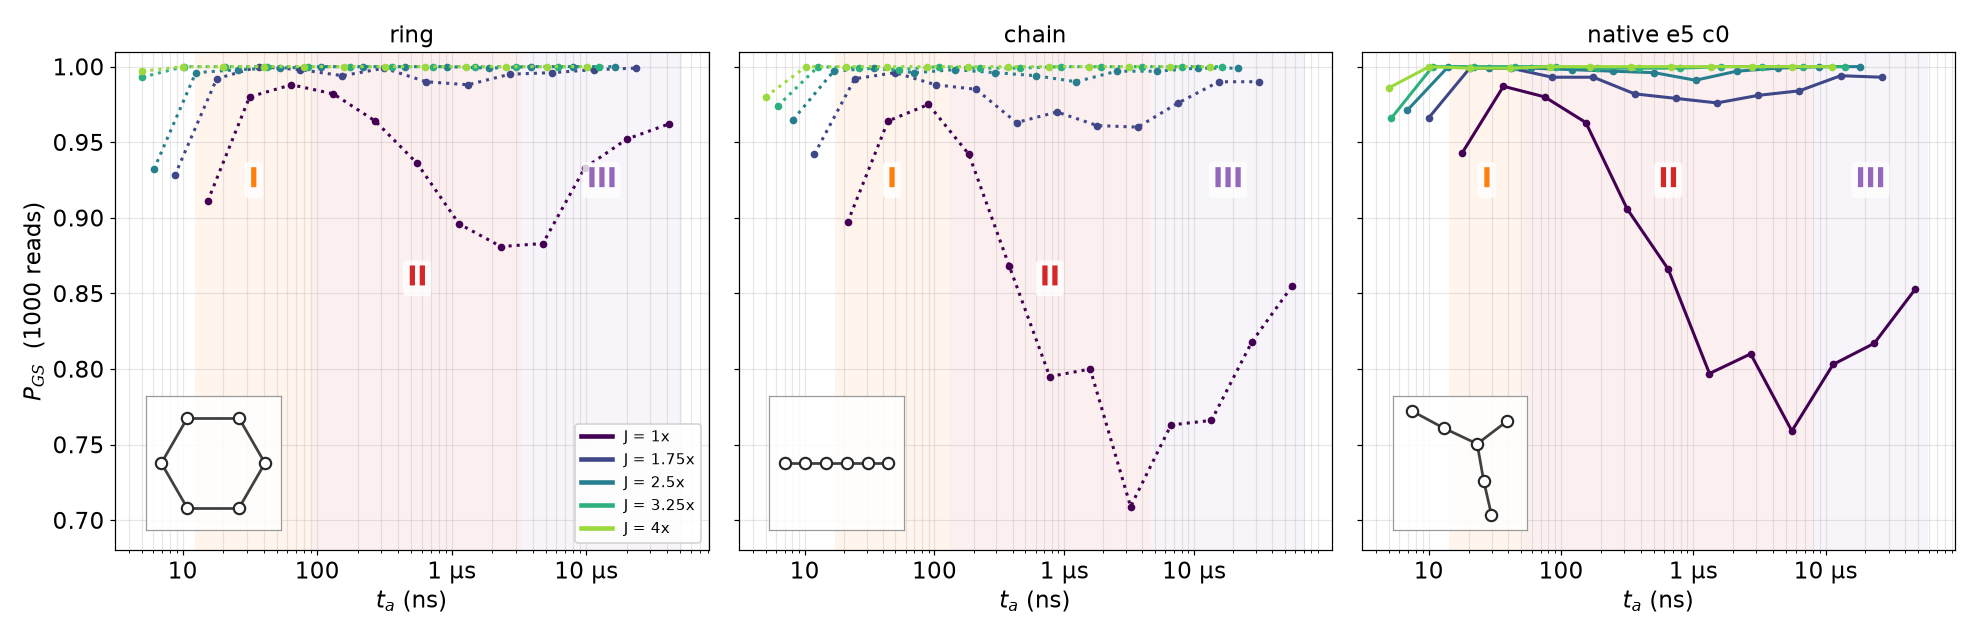
\includegraphics[width=\linewidth]{regimes_three.png}

  \raggedright\small
  
  \textbf{I}: $P_{GS}$ rises with $t_a$ up to a peak at 35--90 ns ($0.975$--$0.988$).
  \textbf{II}: $P_{GS}$ \emph{falls} as the anneal gets slower, to a minimum at 2--6\,$\mu$s ($0.71$--$0.88$) --
  impossible in the ideal case. \textbf{III}: $P_{GS}$ recovers at longer anneals ($0.85$--$0.96$ at 40--57\,$\mu$s).
  Larger $J$ flattens all three. \textbf{The SEAQT comparisons cover 5--145 ns}: regime I, the peak and only the
  first rise of II; ``floor'' in the rest of the talk means this window around the peak.
  \note{The ideal case only knows regime I. Be explicit that the 8000-read data stop at 145 ns, well before the minimum of regime II.}
\end{frame}

\begin{frame}{Large $|J|$: the anneal saturates}
  \centering
  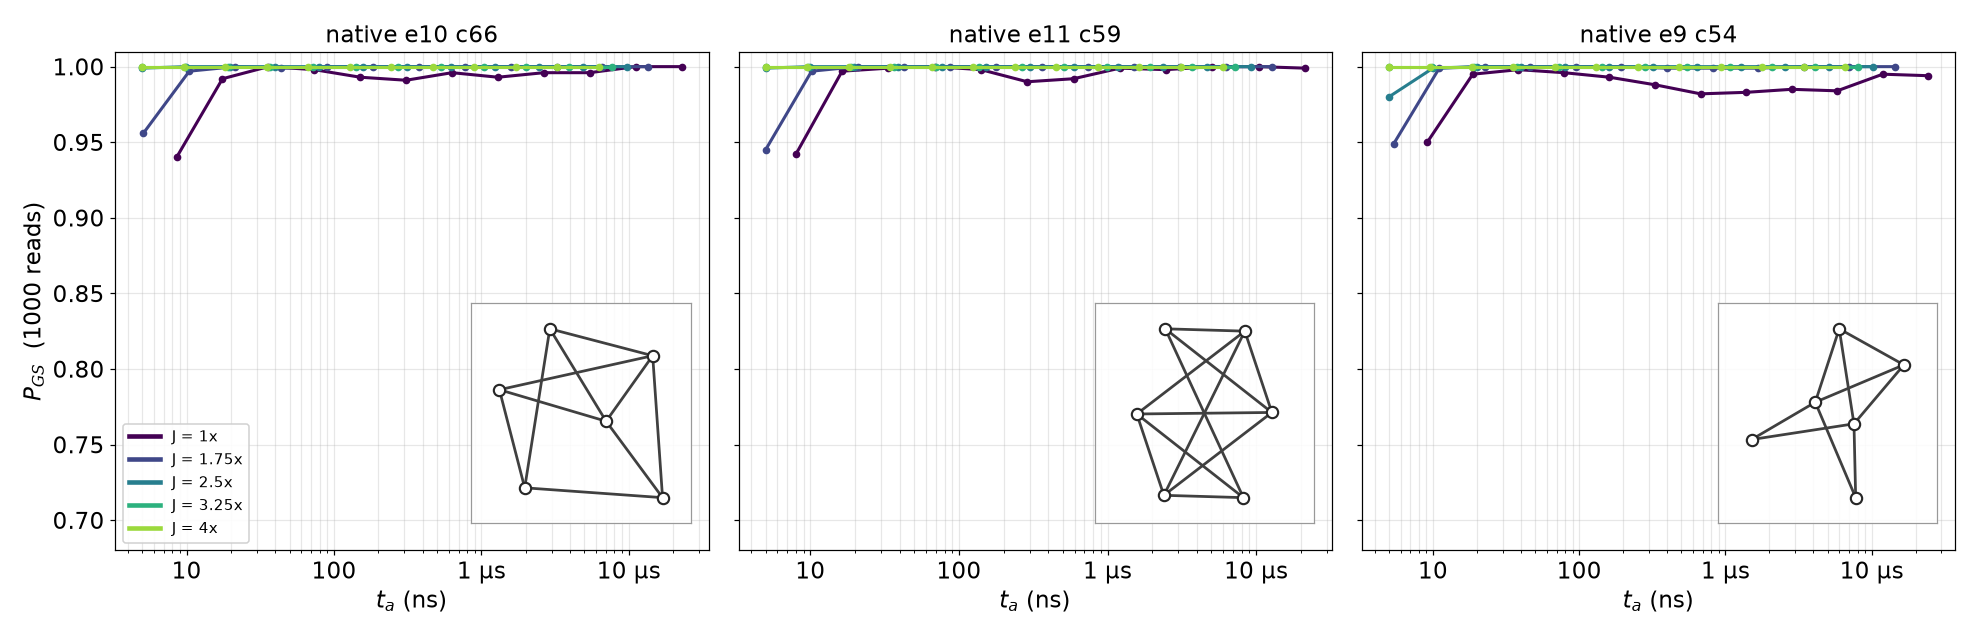
\includegraphics[width=\linewidth]{regimes_saturated.png}

  \raggedright\small
  Densely connected shapes (9--11 couplers among 6 qubits). At $J=1\times$ and $1.75\times$, $P_{GS}$ is below 1 only at
  the shortest anneals ($0.94$--$0.96$, regime I) and then stays $\approx1$: no visible thermal regime. From
  $J=2.5\times$ on, $P_{GS}\ge0.98$ already at 5 ns. Saturated problems (ideal case $>99\%$ at the shortest anneal;
  100 of 215 combinations) carry no information on the dynamics and are left out of the model comparisons.
\end{frame}

\begin{frame}{Frustrated shapes: the sign of $J$ matters}
  \centering
  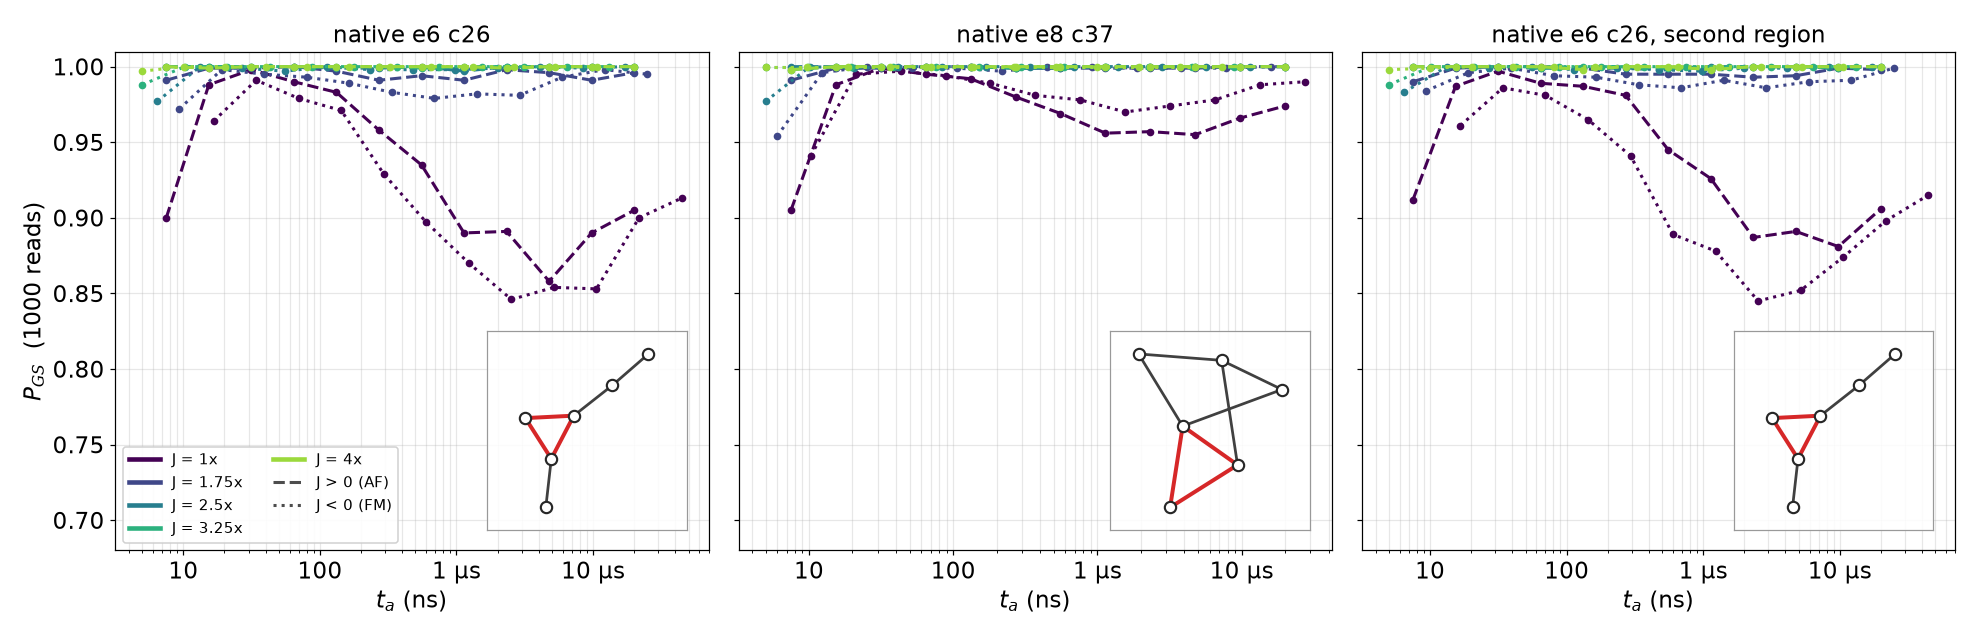
\includegraphics[width=\linewidth]{regimes_frustrated.png}

  \raggedright\small
   Each shape contains one triangle, a loop of 3 qubits: with $J>0$
  (antiferromagnetic) its three couplers cannot all be satisfied at once, so the triangle is frustrated and the ground
  state becomes degenerate (6 states for e6 c26, 4 for e8 c37, instead of 2). The two signs are then genuinely
  different problems -- unlike the ring and chain, where they are gauge-equivalent. At $J=1\times$ the three regimes
  appear for both signs; for e8 c37 regime II is shallow (minimum $0.955$--$0.970$).
\end{frame}

% ------------------------------------------------------------------ 4. hardware reliability
\section{How reliable are the hardware data?}

\begin{frame}{Campaign: the whole chip, repeated over time}
  \begin{itemize}
    \item 616 disjoint 6-cycles tile the chip; every problem runs on all of them at once.
    \item No crosstalk between neighbours: same placements isolated vs.\ surrounded differ by $\le 0.0006$ in $P_{GS}$.
    \item 3 problems (ring $1\times$, chain $1\times$, ring $1.75\times$) $\times$ 2 signs $\times$ 8 anneal times.
    \item 24 complete takes over $\sim$35 h, nominally one per hour.
    \item Three spreads kept apart: \textbf{spatial} (between placements), \textbf{temporal} (between takes,
          within a placement, includes shot noise) and \textbf{chip-wide drift}.
  \end{itemize}
\end{frame}

\begin{frame}{Short anneals: placements differ, time does not}
  \begin{itemize}
    \item At $t_a=5$ ns: spread between placements $2$--$4\times$ the spread between takes
          (ring $1\times$: $0.021$ vs.\ $0.0065$).
    \item Between takes the variation is shot noise (ratio $1.0$--$1.3$); the chip mean changes by $0.05$--$0.09\%$.
    \item The single placement used in earlier campaigns lies within the single-take error bar of the median
          placement: it was representative.
  \end{itemize}
\end{frame}

\begin{frame}{Long anneals: the floor drifts, chip-wide}
  \centering
  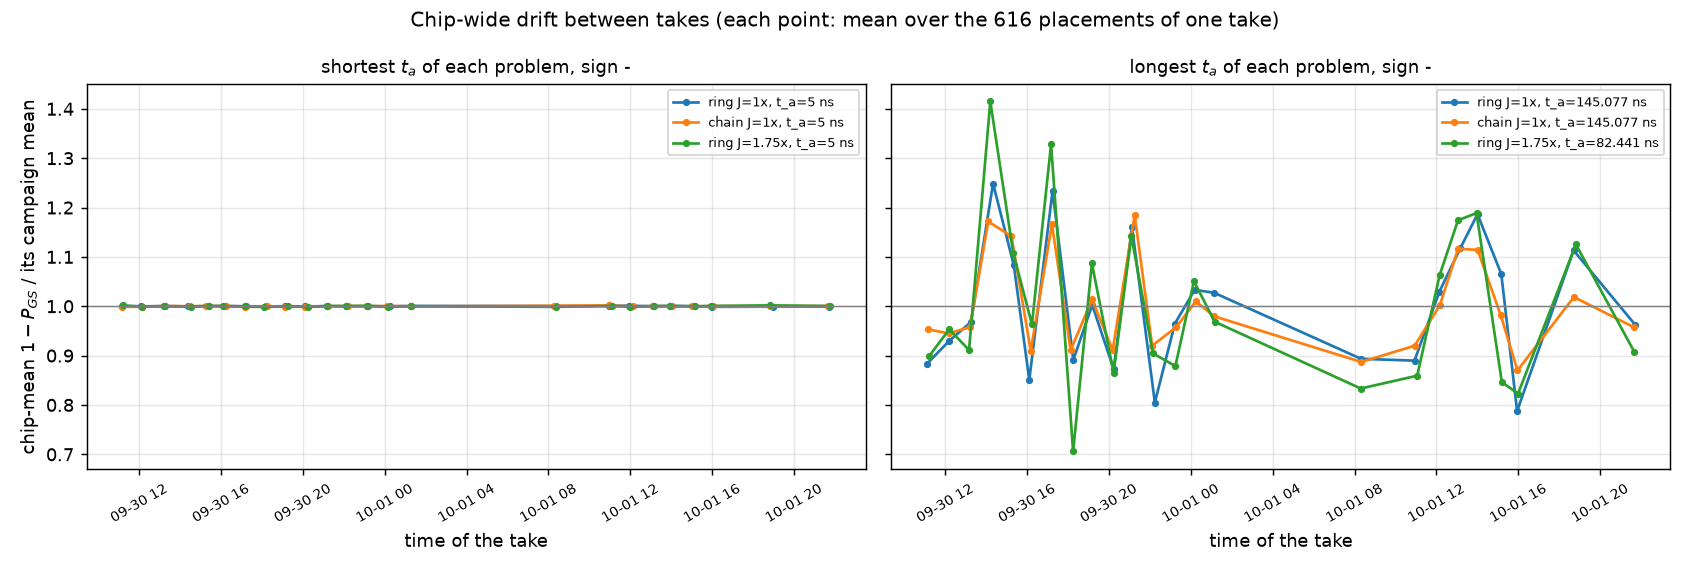
\includegraphics[width=0.95\linewidth]{drift.png}

  \raggedright\small
  Floor ($t_a$ longest): chip mean moves by $10$--$17\%$ (relative std) between takes, range $0.71$--$1.42$;
  the three problems move together; $56$--$77\%$ of the take-to-take variance is shared by all placements
  (ring/chain $1\times$).
  \note{Something chip-wide that affects only the dissipative regime drifts on time scales below an hour.}
\end{frame}

% ------------------------------------------------------------------ 5. unitary
\section{Hardware vs.\ the ideal case}
\begin{frame}{Every hardware point vs.\ ideal case}
  \centering
  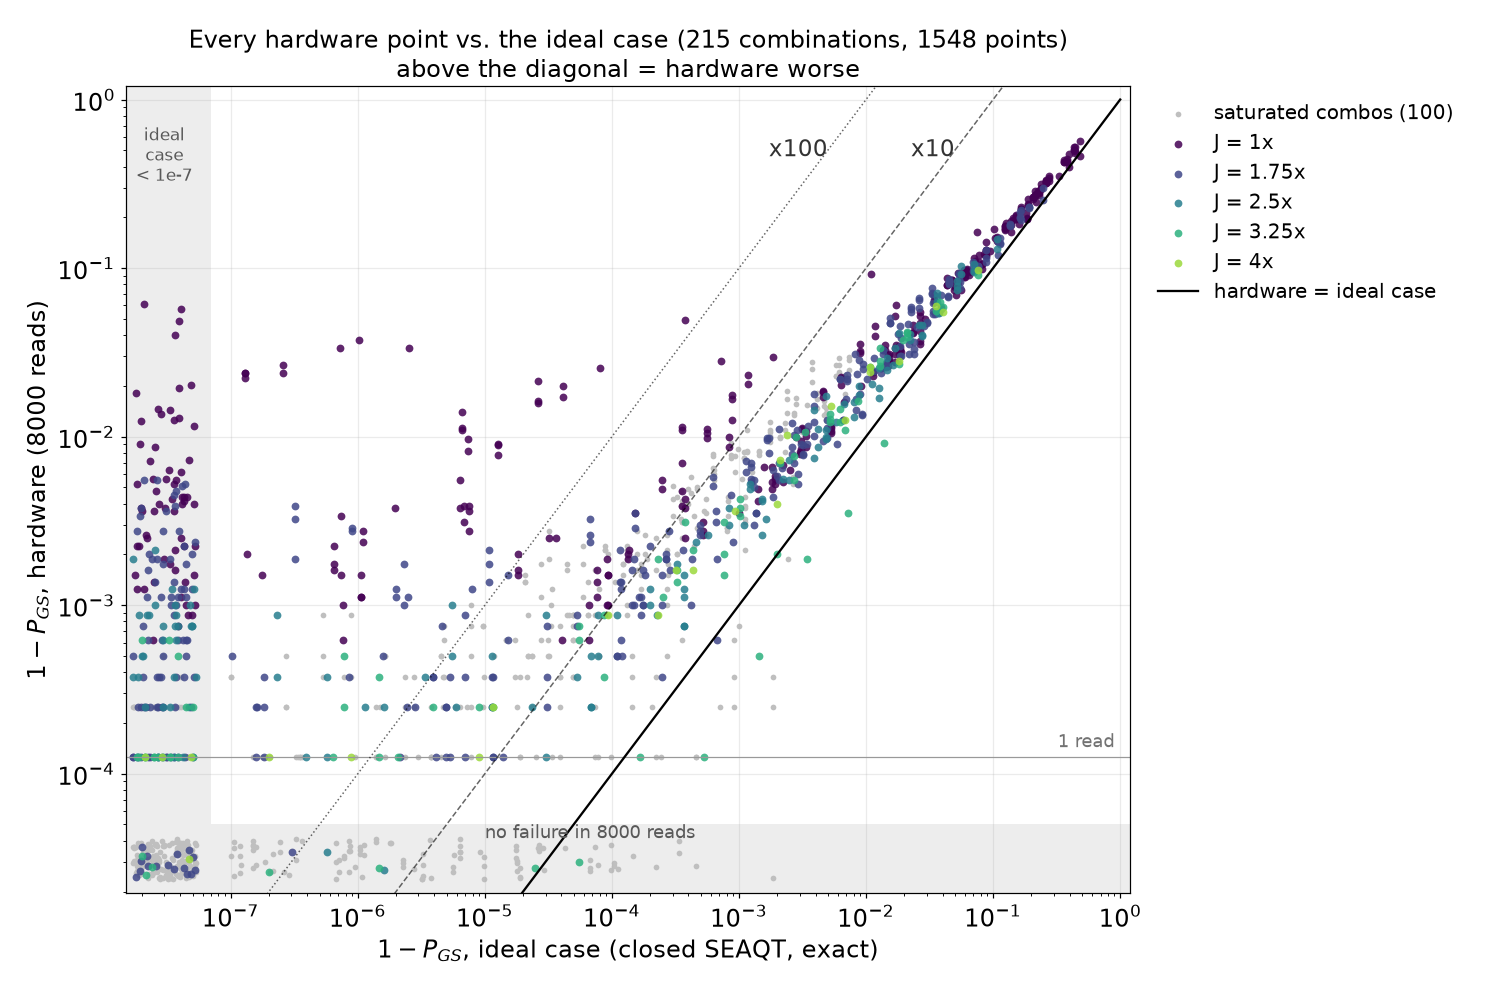
\includegraphics[width=0.8\linewidth]{figures/unitary_scatter_clean.png}
\end{frame}
\begin{frame}{Per shape and coupling: the region barely matters, dense shapes saturate}
  \begin{columns}[c]
    \column{0.5\textwidth}
    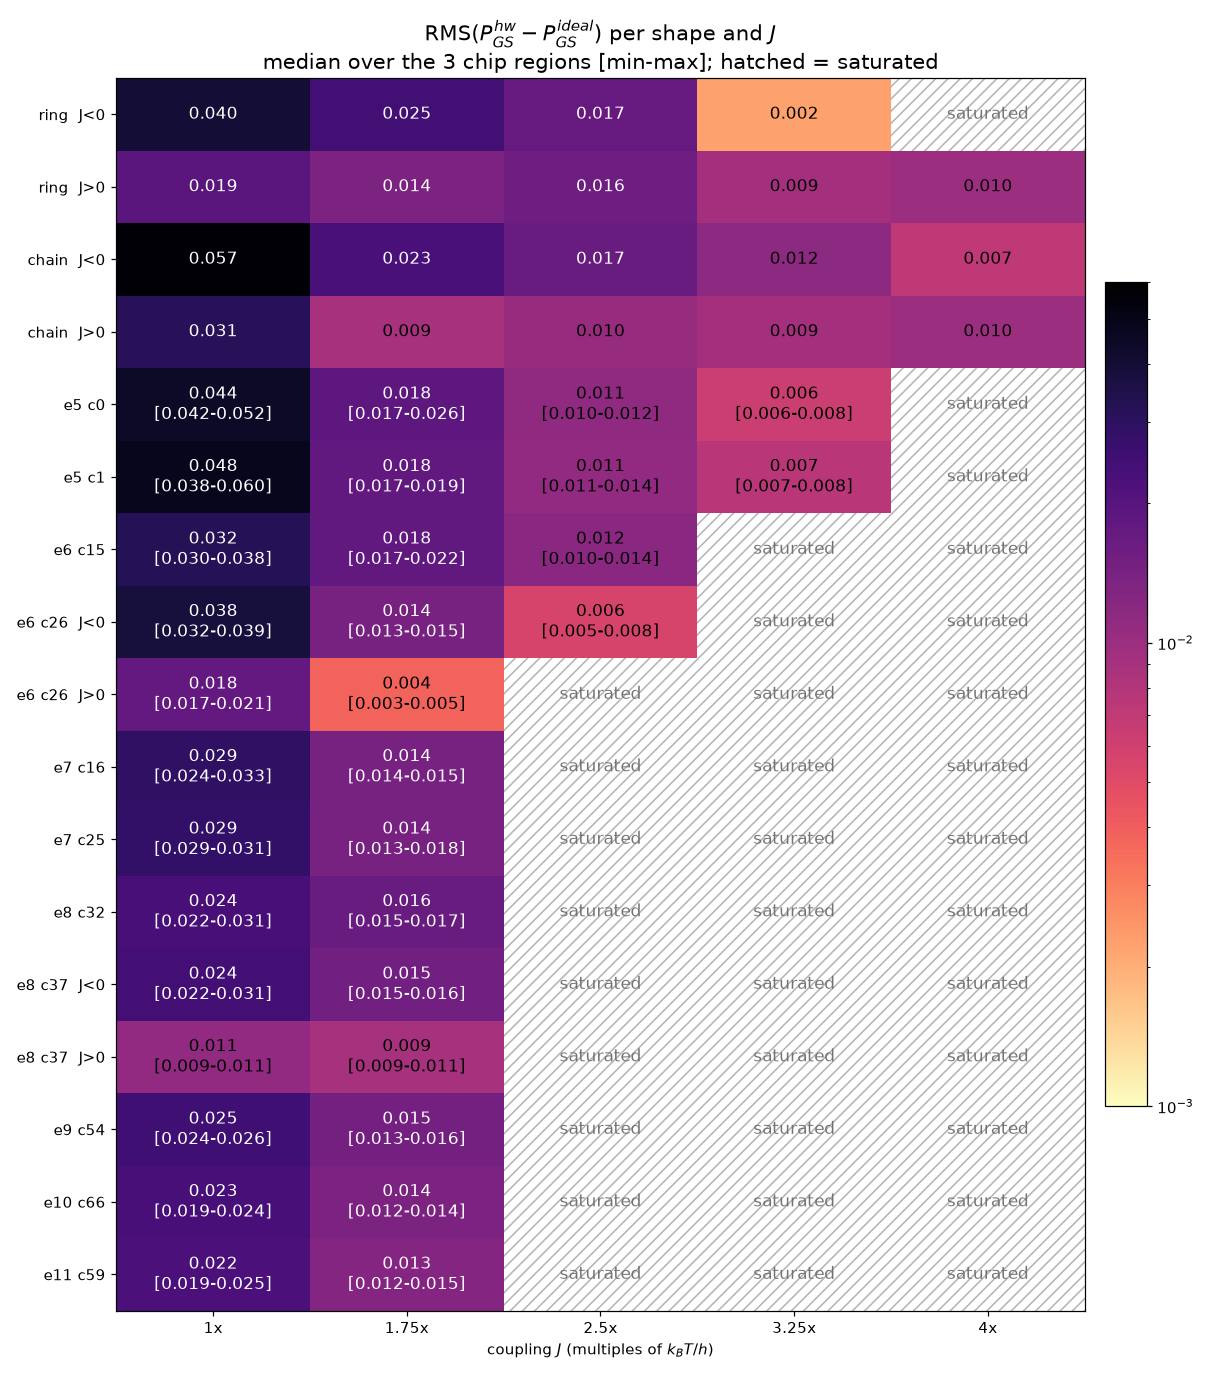
\includegraphics[height=0.86\textheight, width=1.2\textwidth]{unitary_heatmap_regions.png}
    \column{0.48\textwidth}
    \small
    \begin{itemize}
      \item RMS$(P^{hw}-P^{ideal})$ over all $t_a$ of each combination; native shapes measured in 3 chip regions.
      \item Region-to-region range: median $22\%$ of the value (IQR $17$--$34\%$).
      \item Error falls with $J$; it is smaller for $J>0$ than for $J<0$ in every shape measured with both signs.
      \item Saturated (ideal case $>99\%$ at 5 ns) -- the densest shapes from $J=2.5\times$ on.
    \end{itemize}
  \end{columns}
\end{frame}
\begin{frame}{The ideal case follows the coherent regime, misses the floor}
  \centering
  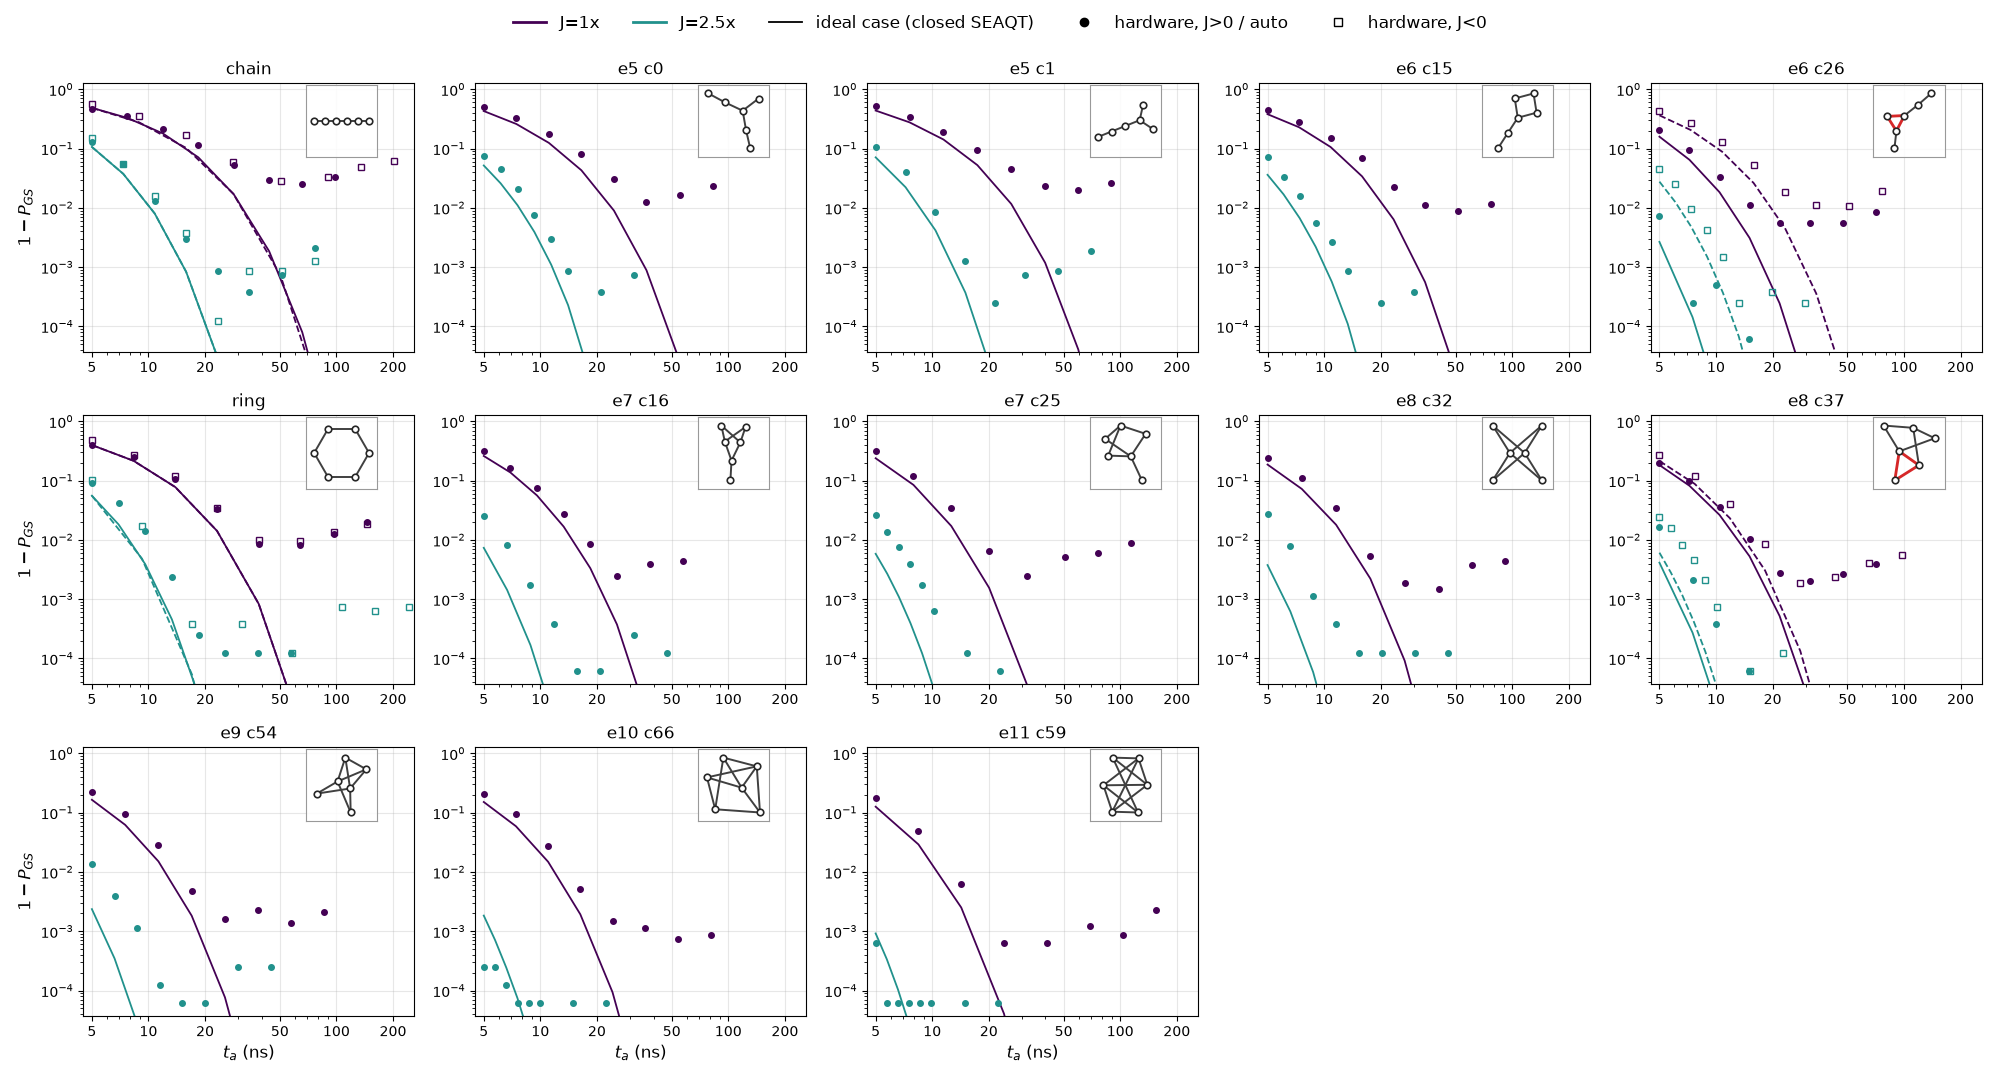
\includegraphics[width=\linewidth]{unitary_13shapes.png}

  \raggedright\small Lines: ideal case; markers: hardware (8000 reads). 13 six-qubit shapes, $J=1\times$ and $2.5\times$.
\end{frame}

\begin{frame}{The coherent excess is chip-wide}
  \begin{columns}[c]
    \column{0.62\textwidth}
    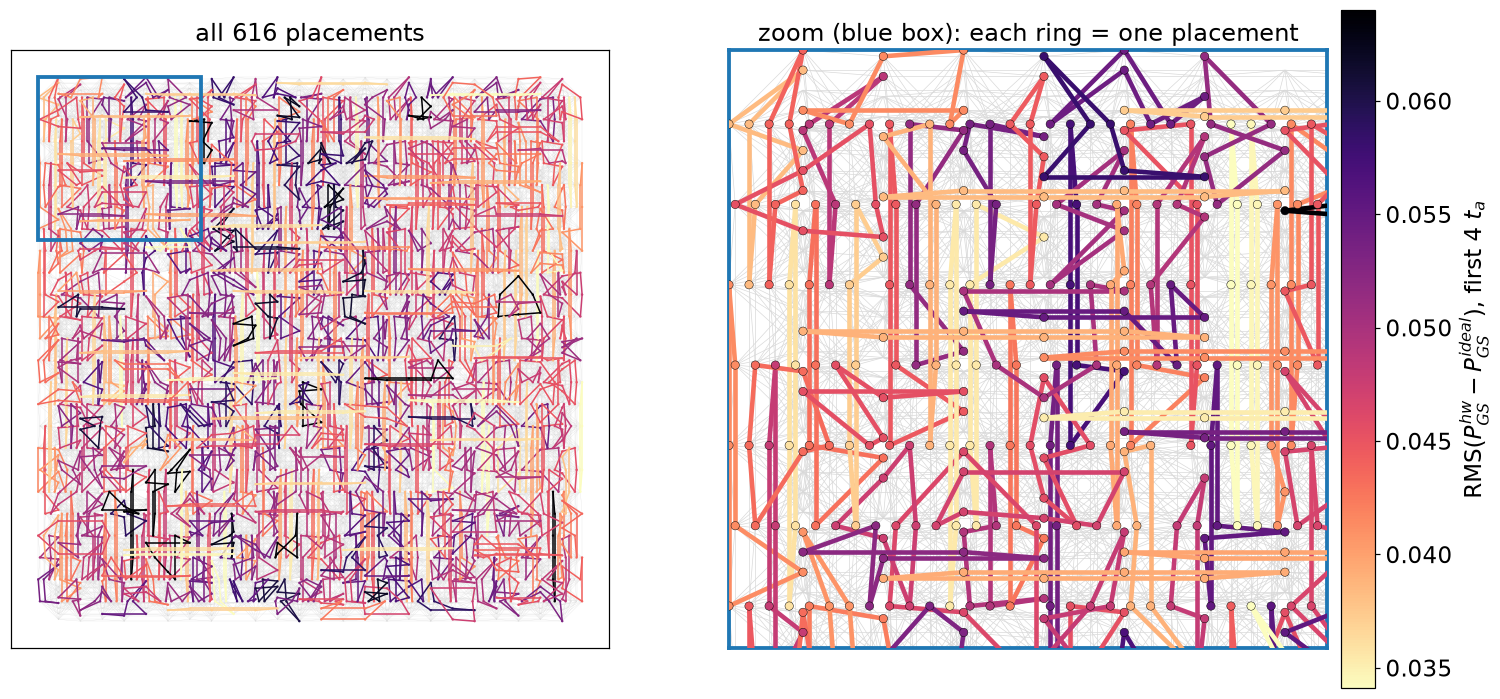
\includegraphics[width=\linewidth]{map_ring1x.png}
    \column{0.36\textwidth}
    \small
    \begin{itemize}
      \item Ring $1\times$, $J<0$: RMS$(P^{hw}-P^{ideal})$ over the first 4 $t_a$.
      \item No placement agrees: $0.038$--$0.057$ (10--90\%).
      \item Real, not noise: odd vs.\ even takes rank placements alike (Spearman $0.97$--$0.99$).
      \item Same placements stand out in all three problems ($0.83$--$0.94$).
    \end{itemize}
  \end{columns}
\end{frame}

\begin{frame}{The coherent deviation depends on the sign of $J$; the floor does not}
  \centering
  \begin{tabular}{@{}lcc@{}}
    \toprule
    Same placement, $J<0$ vs.\ $J>0$ (Spearman) & coherent RMS & floor \\
    \midrule
    ring $1\times$     & $-0.02$ & $0.74$ \\
    chain $1\times$    & $0.01$  & $0.50$ \\
    ring $1.75\times$  & $0.08$  & $0.69$ \\
    \bottomrule
  \end{tabular}
  \vspace{1em}

  \raggedright
  \begin{itemize}
    \item Coherent part: consistent with static per-coupler/qubit calibration errors whose effect flips with sign.
    \item Floor: a sign-independent property of the placement, plausibly thermal.
    \item Zephyr coupler type explains only $8$--$30\%$ of the spatial spread.
  \end{itemize}
\end{frame}

% ------------------------------------------------------------------ 6. dissipators
\section{Hardware vs.\ the two dissipators}

\begin{frame}{Two hypotheses for the floor}
  \begin{columns}[T]
    \column{0.48\textwidth}
    \textbf{Global bath, switched off at $s_c$}
    \begin{itemize}
      \item Whole 6-qubit $\rho$ relaxes to Gibbs$(H(s))$ at 20 mK, rate $w(s)/\tau$.
      \item $w(s)$ switch: logistic at $s_f=0.45$ ($\tau=7$ ns), or a step at the crossing $s_c$ ($\tau=5$ ns).
      \item Positive by construction.
    \end{itemize}
    \column{0.48\textwidth}
    \textbf{Local SEAQT}
    \begin{itemize}
      \item Each qubit relaxes in its locally perceived Hamiltonian.
      \item Calibrated: $T=70$ mK, $\tau=300$ ns.
      \item Fails at the physical 20 mK; no positivity guarantee.
    \end{itemize}
  \end{columns}
  \vspace{1em}
  Both calibrated on the ring $J=1\times$ with the same rule: best floor, coherent RMS $\le 1.1\times$ closed.
\end{frame}

\begin{frame}{Calibration problem: ring $J=1\times$, with error bars}
  \centering
  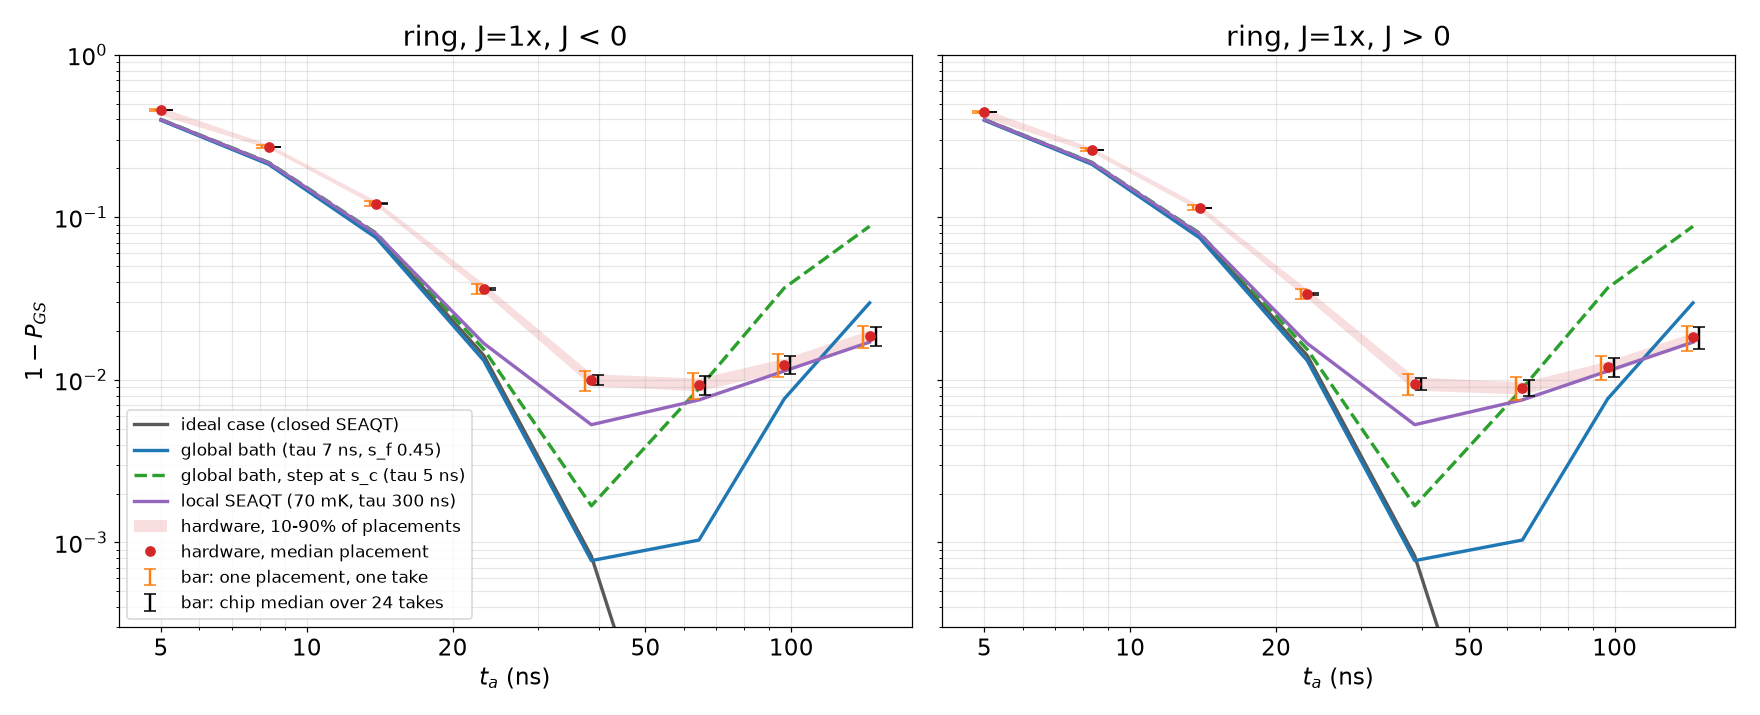
\includegraphics[width=0.92\linewidth]{curves_ring1x.png}

  \raggedright\small Orange bar: one placement, one take. Black: chip median over 24 takes. Band: 10--90\% of placements.
\end{frame}

\begin{frame}{Tests: a new problem, and a new coupling with nothing refitted}
  \centering
  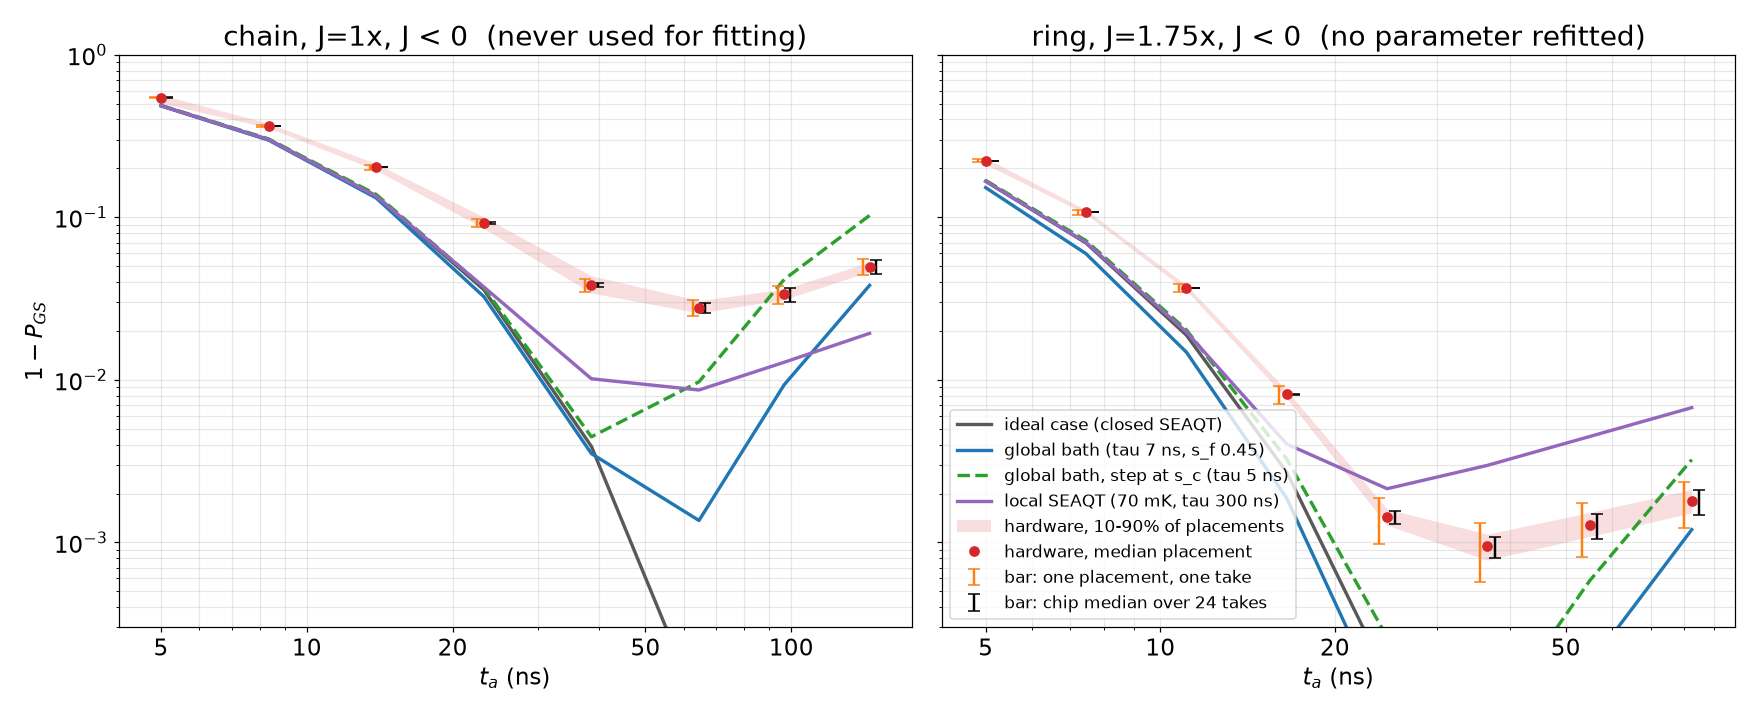
\includegraphics[width=0.92\linewidth]{curves_tests.png}

  \raggedright\small Ring $1.75\times$ with the step at its own $s_c$ and $\tau=5$ ns unchanged:
  error $2.4$--$2.9\times$, vs.\ $108$--$229\times$ for the ideal case.
\end{frame}

\begin{frame}{Across 42 shape/coupling combinations}
  \centering
  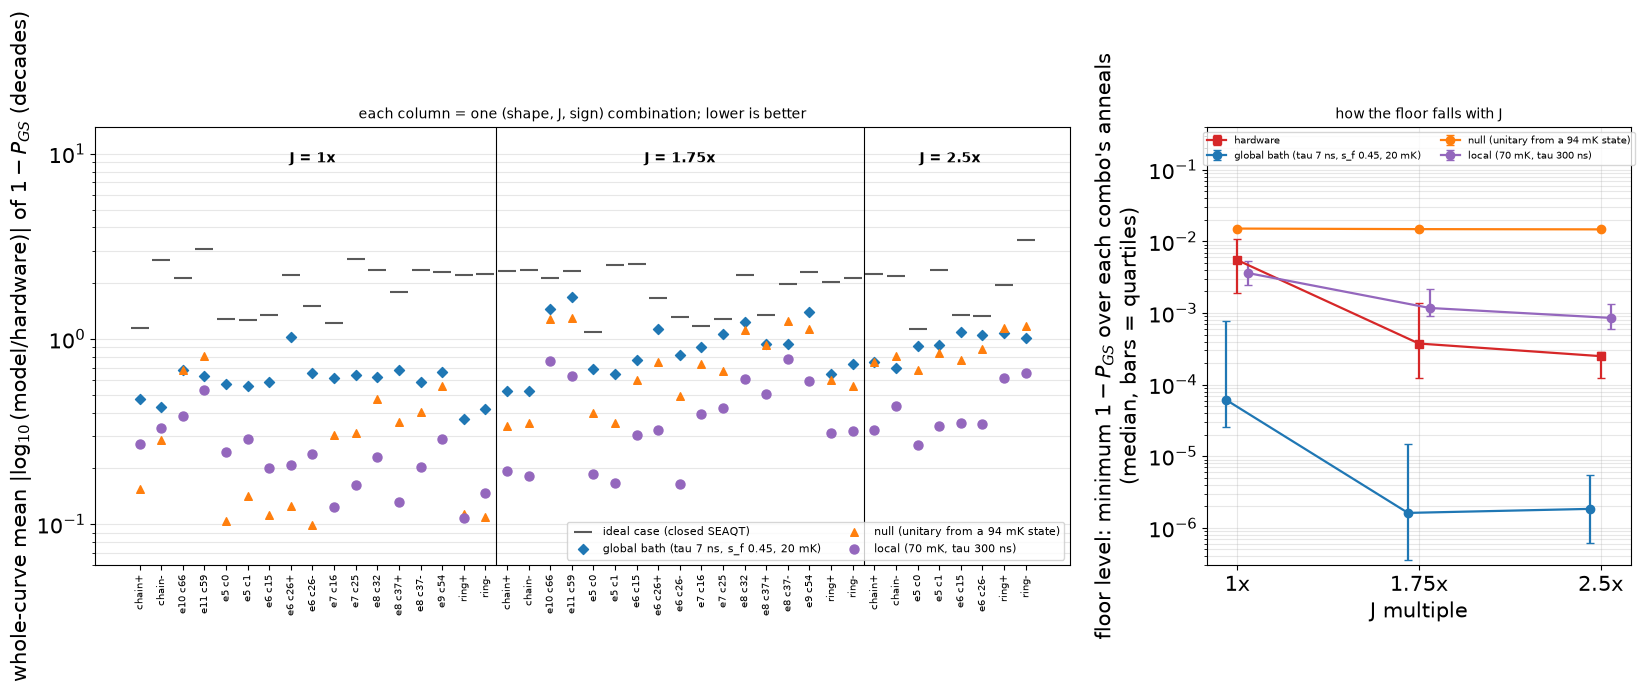
\includegraphics[width=\linewidth]{models_42combos.png}

  \raggedright\small Lower is better. Grey dashes: ideal case. Right: how the floor falls with $J$.
\end{frame}

\begin{frame}{What no dissipator fixes}
  \begin{itemize}
    \item \textbf{Coherent excess.} Hardware $1.4$--$1.9\times$ above the ideal case at short $t_a$: the bath acts after the
          crossing, so it cannot help.
    \item \textbf{Floor level per problem.} Local: right on ring $1\times$ (where calibrated), $3.4\times$ too high on
          ring $1.75\times$, $\sim\!2.7\times$ too low on the chain. Step at $s_c$: most uniform, $1.9$--$3.7\times$.
    \item \textbf{Floor slope.} The model's floor rises $\sim\!11\times$ too fast with $t_a$; a $2\times2$ swap shows
          the pre-$s_c$ bath, not the post-switch tail, is responsible.
    \item \textbf{Temperature.} The local dissipator needs an effective 70 mK, not the physical 20 mK.
  \end{itemize}
\end{frame}

% ------------------------------------------------------------------ 6b. sensitivity to tau
\section{How tightly do the data fix $\tau$?}

\begin{frame}{Where does $\tau$ matter?}
  \begin{itemize}
    \item \textbf{Readout first.} Readout does not depend on $t_a$, so on the same qubits it cannot exceed the smallest
          error measured there: $\le1.9\times10^{-4}$ (ring $2.5\times$ on the 616 placements). The floors are thermal.
    \item \textbf{Elasticity} $E=\partial\ln(1-P)/\partial\ln\tau$: $\approx0$ in the coherent window, $-1$ (local) to
          $-5$ (global) in the floor. All the information on $\tau$ is in the floor.
    \item \textbf{Resolution} $\Delta\tau/\tau\approx$ chip drift$/|E|$: 1--11\% (global), 7--18\% (local).
    \item \textbf{Within a problem $\tau$ is pinned to $\pm$2--18\%}, take to take and placement to placement, with no
          spatial structure.
  \end{itemize}
  \note{The question is not only "which tau" but "what part of the data says anything about tau": only the floor.}
\end{frame}

\begin{frame}{One $\tau$ per problem? Global vs.\ local}
  \centering
  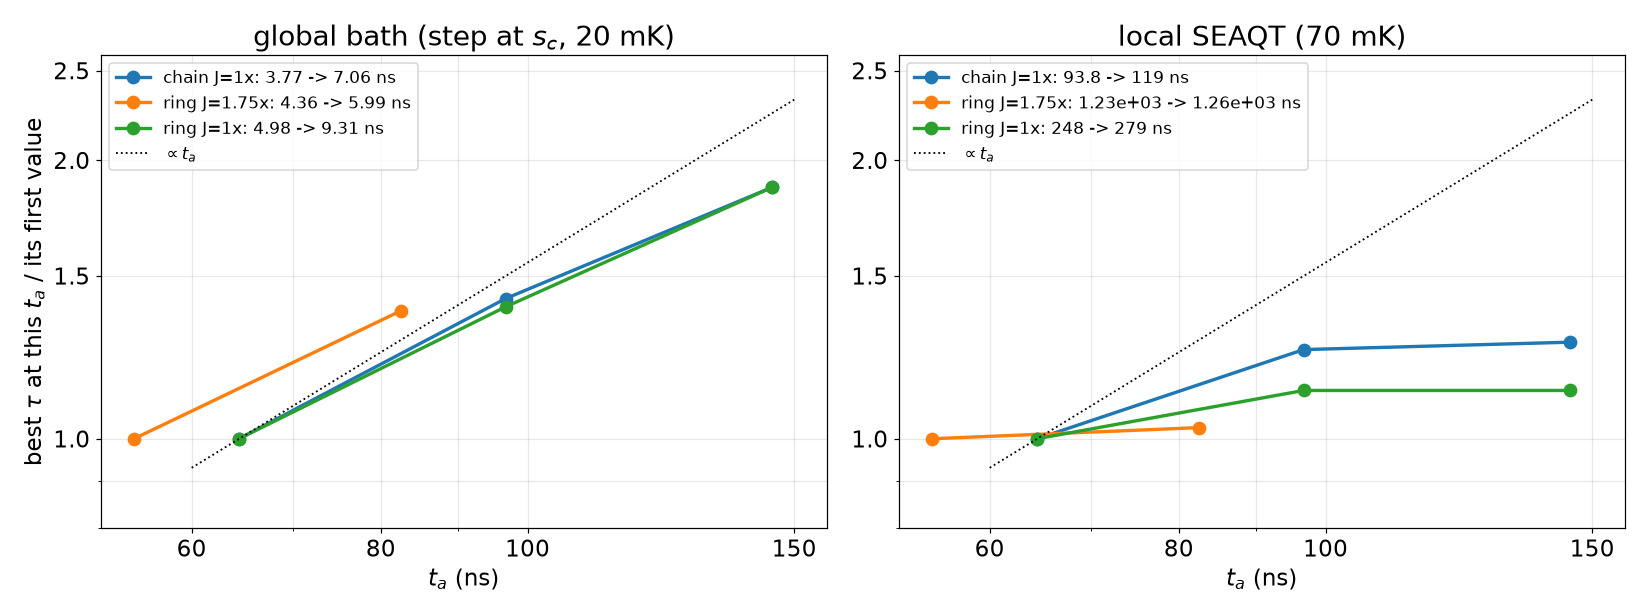
\includegraphics[width=\linewidth]{tau_best_vs_ta.png}

  \raggedright\small
  Best $\tau$ at each $t_a$ on its own. Global: it grows almost $\propto t_a$ (the model compensates a floor that rises
  too fast). Local: nearly constant, exactly as the hardware's own growth predicts. Between problems: global
  3.5--5.6 ns (factor 1.6); local 93 ns (chain), 245 ns (ring $1\times$), 1080 ns (ring $1.75\times$) -- factor $>10$.
\end{frame}

\begin{frame}{A pre-registered test: ring $J=2.5\times$}
  \begin{columns}[c]
    \column{0.6\textwidth}
    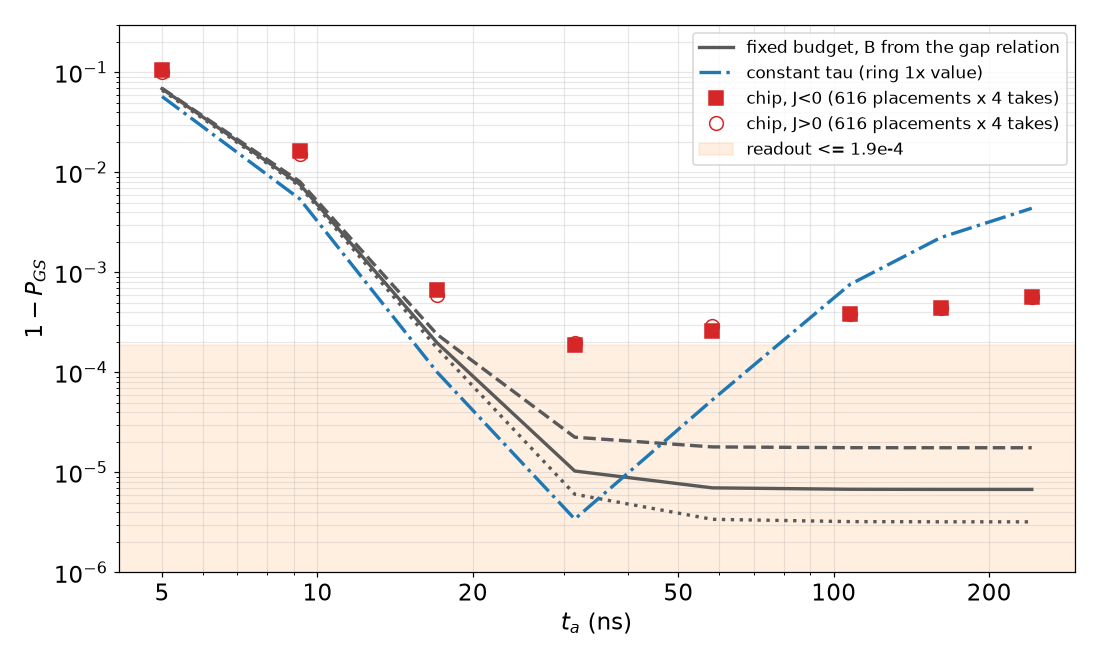
\includegraphics[width=\linewidth]{ring25_prediction_test.png}
    \column{0.38\textwidth}
    \small
    \begin{itemize}
      \item Prediction committed \emph{before} the measurement: fixed relaxation budget from the $B$--gap relation
            (flat floor) and, as alternative, constant $\tau$ (rise $\times80$).
      \item Chip: the floor rises $\times2.0$--$2.2$ from 58 to 242 ns.
      \item \textbf{Both fail}, in trend and in level.
    \end{itemize}
  \end{columns}
  \note{This is the strongest evidence that neither parametrization captures the mechanism. Committed in git before the takes.}
\end{frame}

\begin{frame}{Global and local, side by side}
  \centering\small
  \begin{tabular}{@{}lll@{}}
    \toprule
    & Global (step at $s_c$) & Local \\
    \midrule
    Temperature & 20 mK (physical) & 70 mK (fitted) \\
    $\tau$ between problems & factor 1.6 & factor $>10$ \\
    Floor fit within a problem & 2.4--3.4 (const.\ $\tau$); $\sim$1.3 (fixed budget) & 1.24--1.43 \\
    Floor exponent (hardware 0.70--0.87) & $\sim$2.8 or $\sim$0 & 1.0 \\
    Positivity & guaranteed & violated, $<0.5\%$ of $1-P$ in the floor \\
    Out-of-sample prediction & failed (ring $2.5\times$) & no rule to predict from \\
    \bottomrule
  \end{tabular}
  \vspace{0.8em}

  \raggedright In physical credibility the global bath wins; in the \emph{shape} of the floor the local one wins.
  Both, and the hardware, make only minimum-order errors (one flipped domain).
\end{frame}

\begin{frame}{What the hardware asks for}
  \begin{columns}[c]
    \column{0.6\textwidth}
    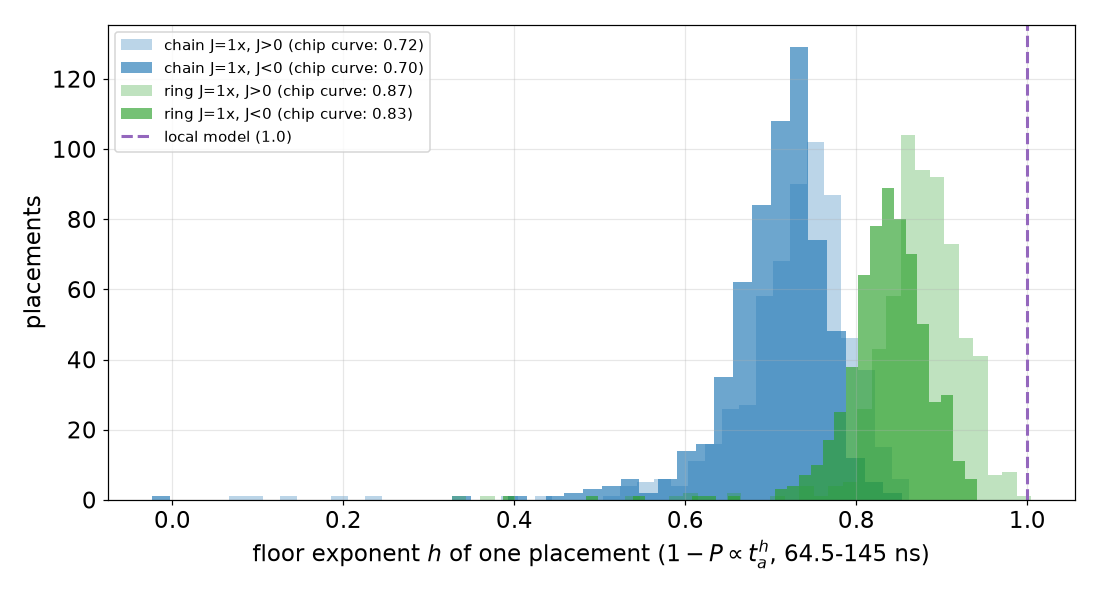
\includegraphics[width=\linewidth]{floor_exponent_hist.png}
    \column{0.38\textwidth}
    \small
    \begin{itemize}
      \item The thermal error grows \textbf{sublinearly}: $1-P\propto t_a^{0.70-0.87}$ in the floor, flattening toward
            the microseconds.
      \item The same exponent in \textbf{every placement} (spread 5--11\%): intrinsic, not an average over a
            heterogeneous chip.
      \item No model has this shape: global too steep or flat, local linear.
    \end{itemize}
  \end{columns}
  \note{Candidates: a broad distribution of relaxation rates within each problem, or low-frequency noise. Untested.}
\end{frame}

% ------------------------------------------------------------------ 7. conclusions
\section{Conclusions}

\begin{frame}{Conclusions}
  \textbf{Where SEAQT predicts well}
  \begin{itemize}
    \item The shape of the coherent regime (validated against King et al.).
    \item The crossing $s_c$ as the point where the bath stops acting: generalizes to a new $|J|$ with zero parameters.
    \item The floor level of a problem, with one parameter.
  \end{itemize}
  \textbf{Where it does not}
  \begin{itemize}
    \item A chip-wide $1.4$--$1.9\times$ excess in the coherent regime.
    \item The floor's weak $t_a$ dependence, and one floor level for all problems.
    \item $\tau$ is pinned to a few \% within a problem, but it is not a property of the chip: a pre-registered
          prediction for a new problem failed.
  \end{itemize}
  \textbf{Data quality}: the comparison holds over 616 placements and 24 takes; the floor drifts by $10$--$17\%$.
\end{frame}

\begin{frame}{Open questions}
  \begin{itemize}
    \item What produces the sublinear growth $t_a^{0.7-0.9}$, identical in every placement: a distribution of
          relaxation rates, or low-frequency noise?
    \item Which single-domain states does the chip populate? (needs bitstrings; the models are ready)
    \item Can a topological speed limit bound $\tau$ independently of the fit? (thesis project)
    \item Per-qubit $\tau_J$ in the local model, compared with per-coupler data from the chip.
    \item What drives the chip-wide floor drift: effective temperature, bath coupling?
  \end{itemize}
\end{frame}

\begin{frame}[standout]
  Thank you -- questions?
\end{frame}

% ------------------------------------------------------------------ backup
\appendix
\section*{Backup}



\begin{frame}{Backup: calibration scans of both dissipators (ring $1\times$)}
  \centering
  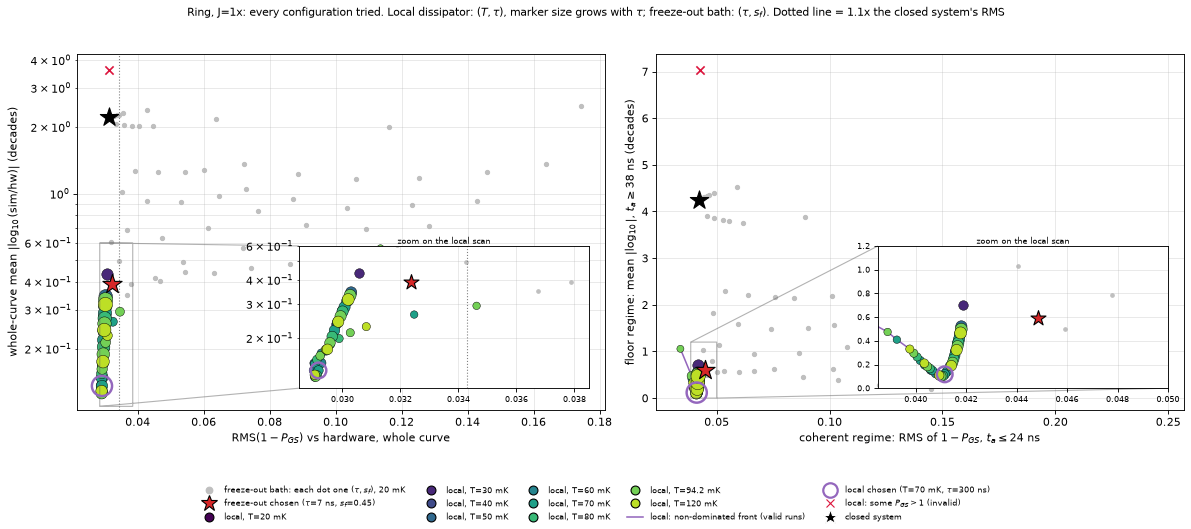
\includegraphics[width=\linewidth]{calibration_scan.png}
\end{frame}

\begin{frame}{Backup: quasi-staticity at $s_c$ (Marshall, Rieffel \& Hen)}
  \begin{columns}[c]
    \column{0.55\textwidth}
    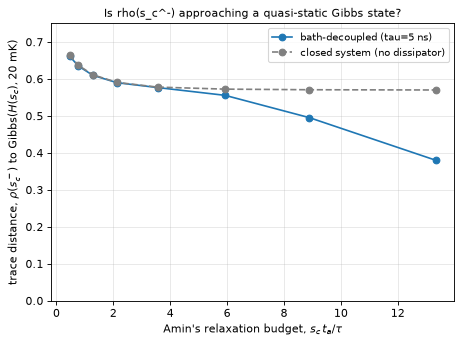
\includegraphics[width=\linewidth]{quasistaticity.png}
    \column{0.42\textwidth}
    \small
    \begin{itemize}
      \item Trace distance to Gibbs$(H(s_c))$ falls $0.66\to0.38$ with the relaxation budget, but never reaches 0.
      \item Coherences collapse ($1.10\to0.05$); populations stay at $0.51$--$0.55$.
      \item So: a bath-decoupling point, not yet a freeze-out in Amin's sense.
    \end{itemize}
  \end{columns}
\end{frame}

\begin{frame}{Backup: dependence on Zephyr coupler type}
  \centering
  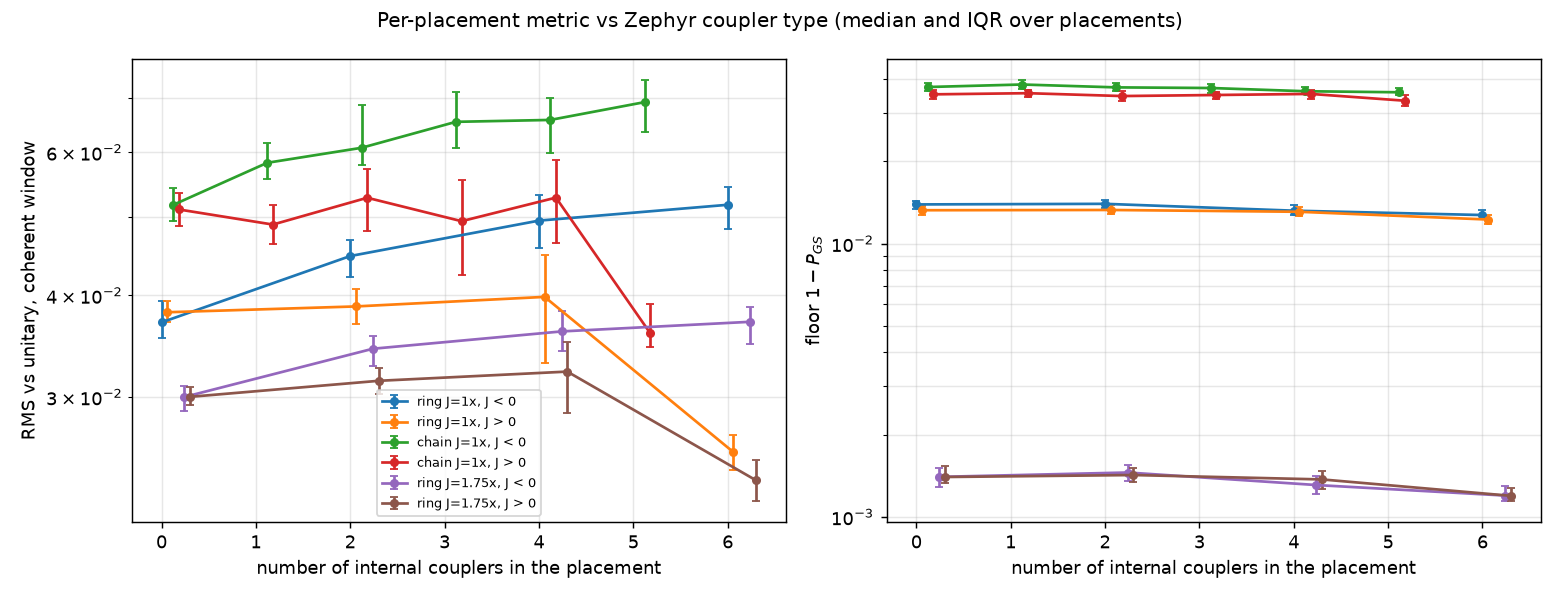
\includegraphics[width=\linewidth]{coupler_type.png}
\end{frame}

\begin{frame}{Backup: all models, including the null model}
  \centering
  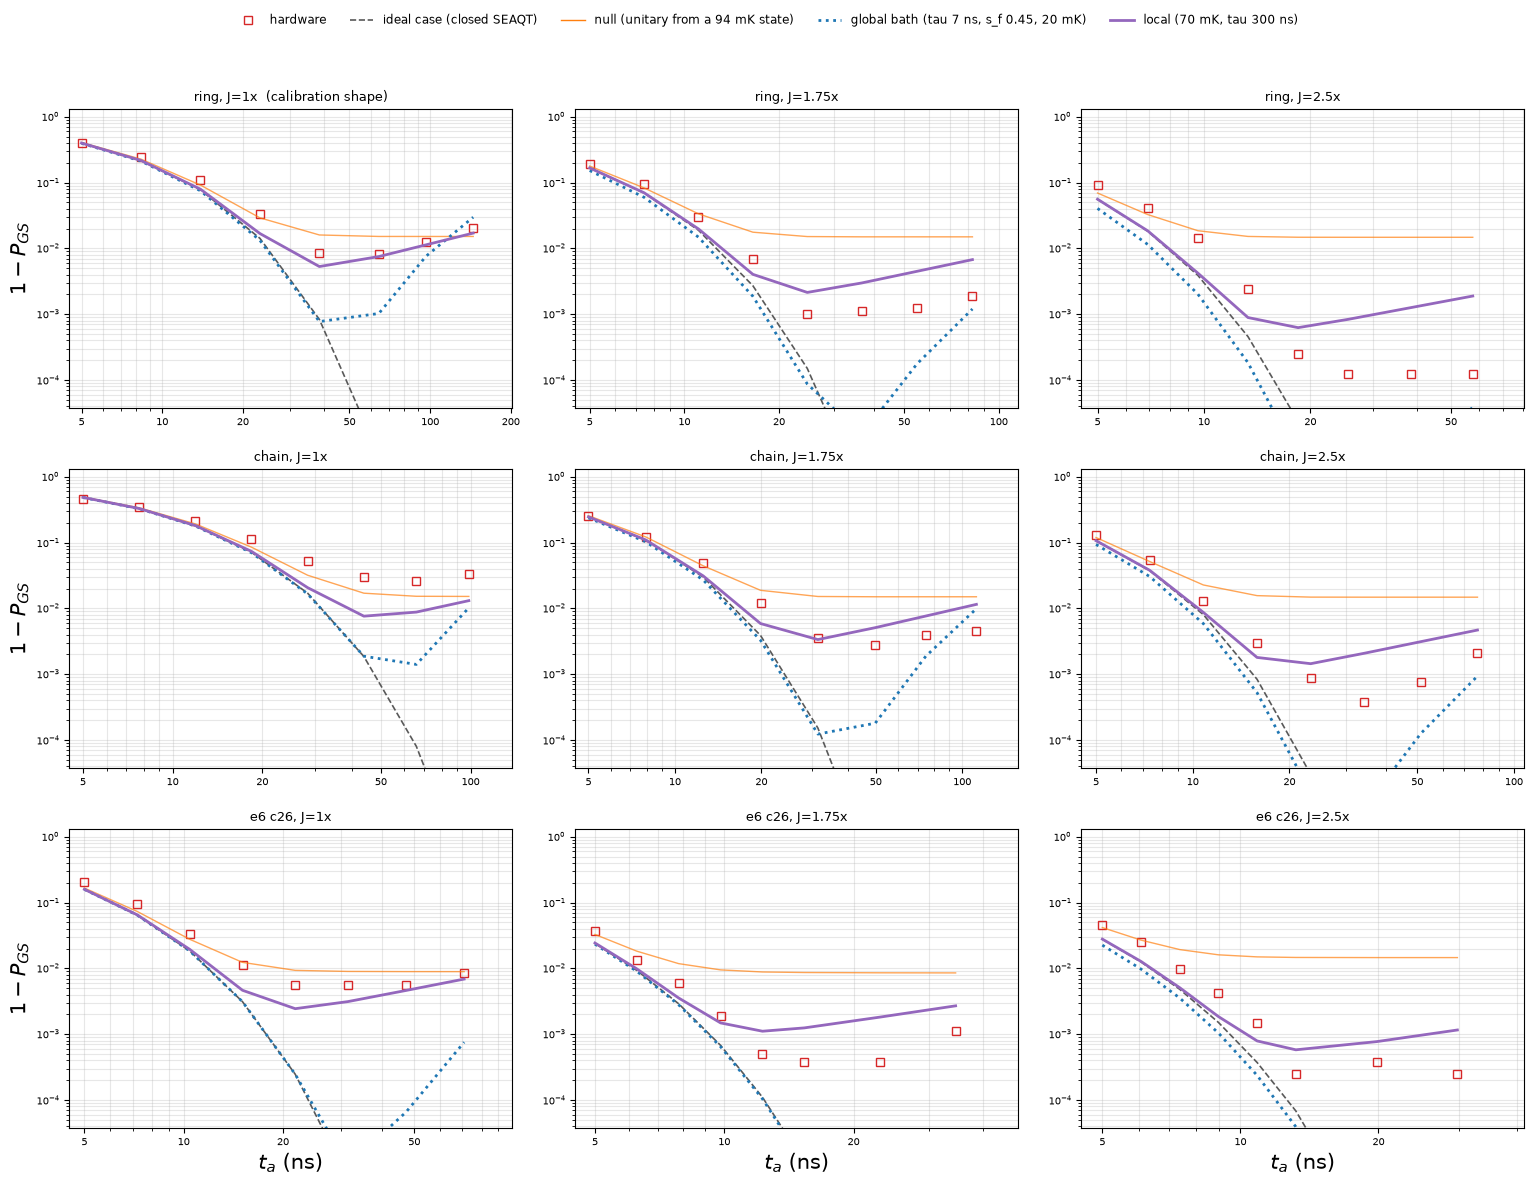
\includegraphics[height=0.82\textheight]{models_curves_grid.png}

  \raggedright\small Null model: unitary evolution from a 94 mK Gibbs state; its floor is the initial excited population.
\end{frame}

\end{document}
